% This file was created with tikzplotlib v0.10.1.
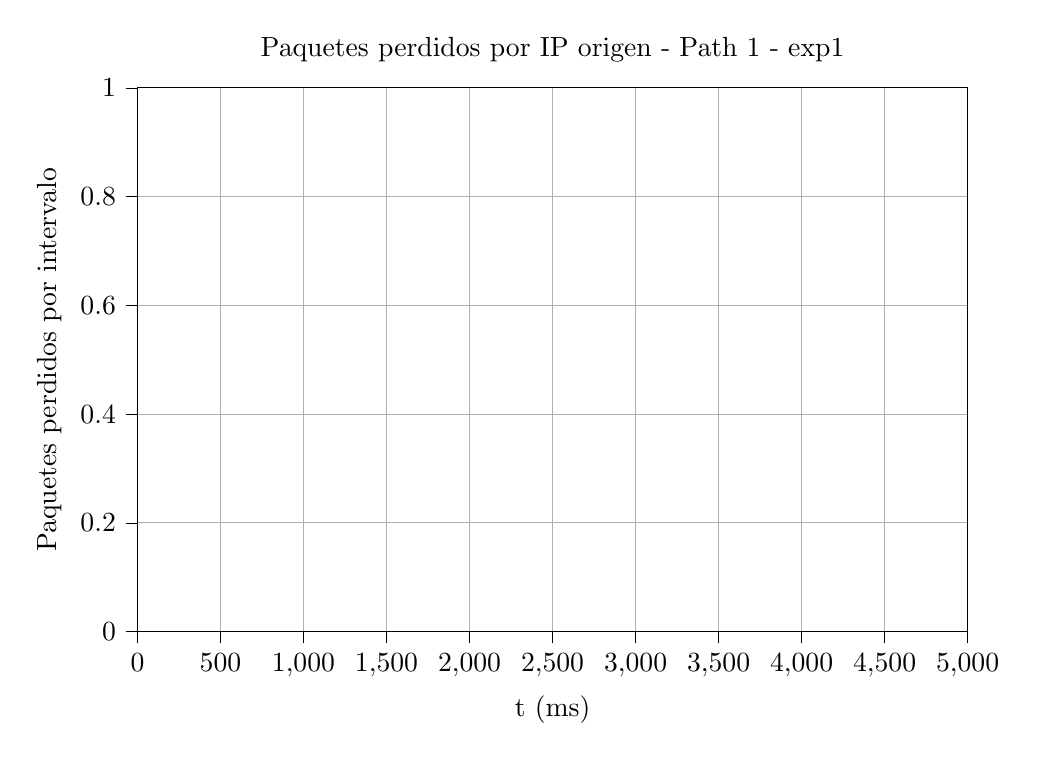
\begin{tikzpicture}

\definecolor{darkgray176}{RGB}{176,176,176}

\begin{axis}[
height=0.7\textwidth,
tick align=outside,
tick pos=left,
title={Paquetes perdidos por IP origen - Path 1 - exp1},
width=\textwidth,
x grid style={darkgray176},
xlabel={t (ms)},
xmajorgrids,
xmin=0, xmax=5000,
xtick style={color=black},
y grid style={darkgray176},
ylabel={Paquetes perdidos por intervalo},
ymajorgrids,
ymin=0, ymax=1,
ytick style={color=black}
]
\end{axis}

\end{tikzpicture}
